\section{Sampling}
\label{Chap:Sampling}
\begin{frame}[t]{Chapter \autoref{Chap:Sampling}}
\tableofcontents[sections= \value{section}]
\end{frame}


\begin{frame}[t]{Sampling}

\begin{itemize}

\item Sampling allow continuous time signals to processed through discrete time signal

\item Question to be asked during sampling: 

how fast do we need to sample, and for how long ?

\item Study effect of sampling in frequency domain using Fourier Analysis

	\begin{itemize}
	\item See its effect on the spectrum of the original signal
	
	\item How we can recover the original signal
	\end{itemize}


\item Effect of Quantization didn't cover it yet (to be done later)

\end{itemize}



\end{frame}


\subsection{Ideal (Impulse) Sampling}
\label{Sub:Ideal_Sampling}


\begin{frame}[t,allowframebreaks]{Impulse Sampling}


\begin{itemize}

\item  Spectrum is replicated at multiple of $\omega_s$ \cite{signal_processing_Lathi}

\begin{equation}
X_{\delta}(\omega) \, = \, \displaystyle\frac{1}{T_s} \displaystyle\sum\limits_{k \, = \, -\infty}^{+ \infty} X_c \left(\, \omega \, - \, k \,\omega_s  \,\right)
\end{equation}

\item  When \textcolor{red}{sampling higher then the Nyquist rate}, we could still distinguish the original version of the spectrum, which is in the middle

\item \textcolor{red}{Decreasing the sampling rate}: distortion of the original spectrum due to the overlapping among the replication \ref{Sub:Ideal_Sampling}

	\begin{itemize}
	\item This effect is know as \textcolor{red}{aliasing}
	\end{itemize}

\end{itemize}

\begin{figure}[ht]
\centering
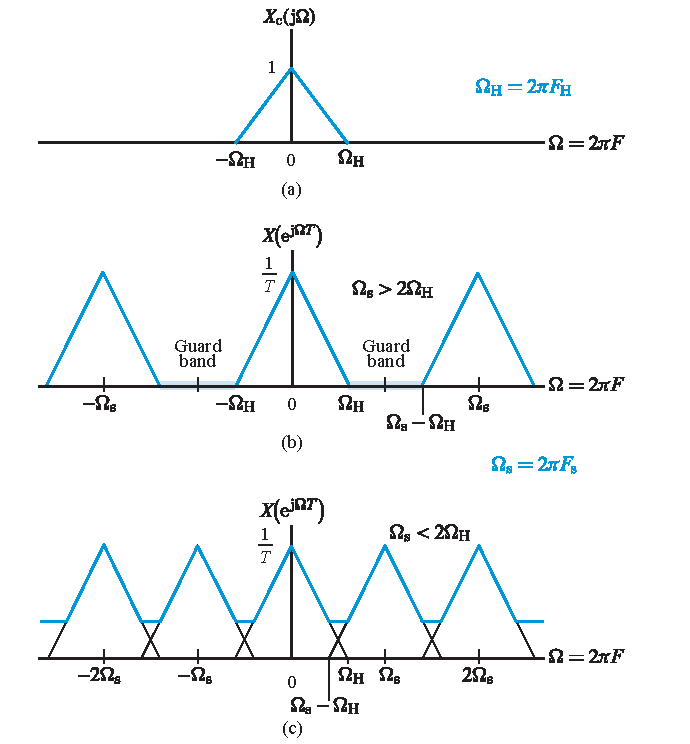
\includegraphics[scale=0.4]{Figures/Sampling/Impulse_Sampling_Effect}
\caption{Impulse Sampling Effect in the frequency spectrum \cite{DSP_DimitrisManolakis}}
\label{fig:Sampling:impulse_sampling_spectrum_1}
\end{figure}


\end{frame}


\subsection{Terminology and Definitions in Sampling}

\begin{frame}[t,allowframebreaks]{Terminology in Sampling Operation \cite{DSP_DimitrisManolakis}}

\begin{figure}[ht]
\centering
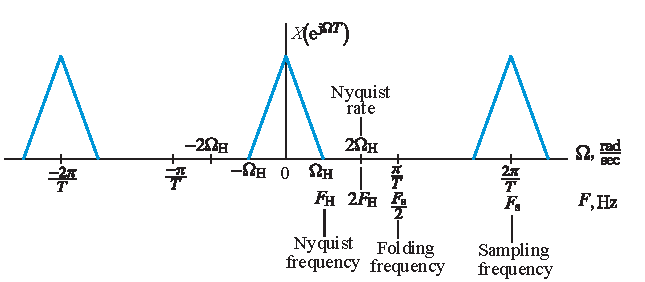
\includegraphics[scale=0.9]{Figures/Sampling/Impulse_Sampling_Terminology}
\caption{Replicated Amplitude Spectrum: Frequency axis in $F$[Hz] and $\omega_c$[rad/s] \cite{DSP_DimitrisManolakis}}
\label{fig:Sampling:Impulse_Sampling_Terminology}
\end{figure}

\newpage
\begin{itemize}

\item Highest Frequency $F_H$ in Hz presented in the continuous time signal $x_c(t) \rightarrow$ \textcolor{red}{Nyquist Frequency}

\item \textcolor{red}{Minimum sampling frequency} required to avoid overlapping bands $\rightarrow$ \textcolor{red}{Nyquist Rate}

\item Actual highest frequency that the sampled signal $x[n]$ contains is $\displaystyle\frac{F_s}{2} \, \rightarrow$ \textcolor{red}{folding frequency} 
 
\end{itemize}

\end{frame}


\subsection{Sampling Example}
\begin{frame}[t]{Sampling Effect Example}

To regenerate the pictures later.

\end{frame}

\subsubsection{Aliasing of Cos Signal}

\begin{frame}[t,allowframebreaks]{Aliasing of Cos Signal}

\begin{figure}[ht]
\centering
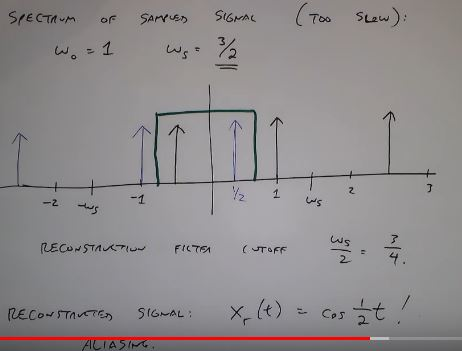
\includegraphics[scale=0.6]{Figures/Sampling/cos_signal_aliasing}
\label{fig:Sampling:cos_aliasing}
\end{figure}

\newpage
\begin{itemize}

\item The low pass filter is from $\displaystyle\frac{-\omega_s}{2} \, \rightarrow \, + \, \displaystyle\frac{+\omega_s}{2}$

\item Because we undersampled (not respect the Nyquist criterion), the DAC construct an aliased cos signal

\end{itemize}


\end{frame}

\subsection{Reconstruction}
\begin{frame}[t,allowframebreaks]{Reconstruction of Baseband Continuous time signal}

\begin{itemize}
\item Goal now: \textcolor{red}{restore} our \textcolor{red}{original signal} from our samples
	
	\begin{itemize}
	\item In other words, undo the effect of sampling
	\end{itemize}

\begin{figure}[ht]
\centering
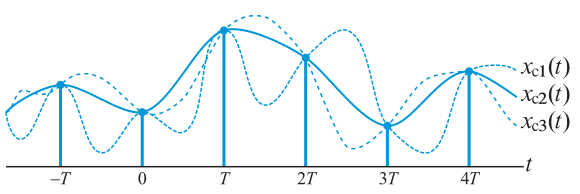
\includegraphics[scale=0.550]{Figures/Sampling/reconstruction_problem}
\caption{Reconstruction from samples: which version to choose \cite{DSP_DimitrisManolakis}}
\end{figure}

\item Working Conditions:

	\begin{itemize}
	\item Assuming that the signal is \textcolor{red}{bandlimited}

	\item Practicle sampling and reconstruction to be done later (like ZOH)
		
	\item Neglecting the effect of quantization for now
	
	
	\end{itemize}

\item This can be done from frequency domain perspective:

	\begin{itemize}
	\item Filtering the original spectrum and reject the images (replications)
	
	\end{itemize}

\item After the proof (to be put later in details) we get:
	
	\begin{equation}
	\hat{x}_{\text{sinc}}(t) \, = \, \displaystyle\sum\limits_{n \, = \, -\infty}^{+ \infty} x_{\text{sampled}} \left(\, n \, T_s \, \right) \text{sinc}\left[\, \displaystyle\frac{\omega_s \, \left(\, t \, - \,  n \, T_s \,\right)}{2}    \,\right]
	\label{Eq:Sampling:Ideal_Reconstruction}
	\end{equation}
	
	\begin{itemize}
	\item $\hat{x}_{\text{sinc}}(t)$ is the \textcolor{red}{sum of shifted sinc}, each \textcolor{red} {weighted} by a different amplitude $x(n \, T_s)$
	\end{itemize}

\end{itemize}

\end{frame}

\begin{frame}[t]{Visual Interpretation of Ideal Reconstruction 1}

\begin{figure}[ht]
\centering
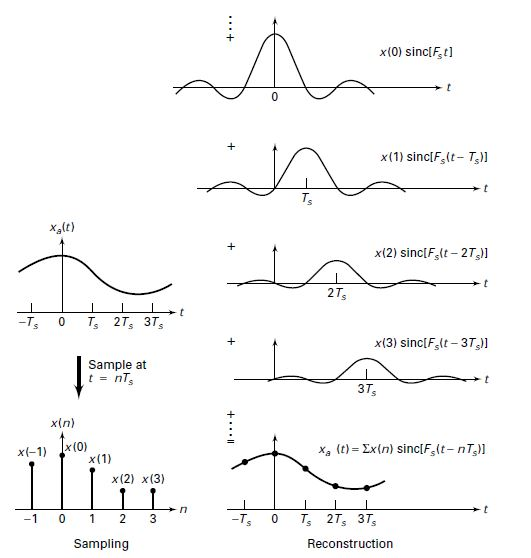
\includegraphics[scale = 0.4]{Figures/Sampling/ideal_bandlimited_interpolation_1}
\caption{Reconstruction of band-limited signal from its samples \cite{DSP_Matlab_Proakis}}
\end{figure}

\end{frame}

\begin{frame}[t]{Visual Interpretation of Ideal Reconstruction 2}

\begin{figure}[ht]
\centering
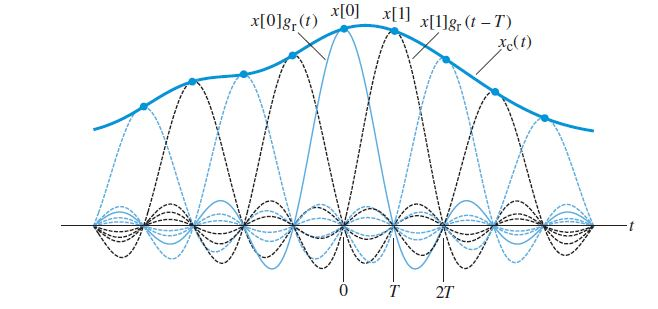
\includegraphics[scale=0.550]{Figures/Sampling/ideal_bandlimited_interpolation}
\caption{Ideal bandlimited interpolation in the time domain \cite{DSP_DimitrisManolakis}}
\end{figure}

\end{frame}


\subsection{Excercice On Ideal Sinc Interpolation}

\begin{frame}[t,fragile]{Implementation of Sinc Interpolation}

\begin{itemize}

\item If we want to implement equation (\autoref{Eq:Sampling:Ideal_Reconstruction}), we need to take care of 2 points:

	\begin{itemize}
	\item The Summation limit: we can't add from $-\infty \rightarrow \, +\infty$, so we need to truncate and choose some grid of discrete samples from $n \, = n_{\text{start} } \rightarrow n_{\text{finish} }$
	
	\item The $t$ is also need to be discretized on some grid: $t \, \approx \,$ \verb|t-start:step:t-end|
	\end{itemize}

\end{itemize}

\end{frame}


\subsection{Practical Reconstruction}
\begin{frame}[t,allowframebreaks]{Practical Reconstruction}

\begin{itemize}

\item Recap: Ideal reconstruction is done based on infinite sum of interpolated sinc 

\begin{equation}
	\hat{x}(t) \, = \, \displaystyle\sum\limits_{n \, = \, -\infty}^{+ \infty} x\left(\, n \, T_s \, \right) \text{sinc}\left[\, \displaystyle\frac{\omega_s \, \left(\, t \, - \,  n \, T_s \,\right)}{2}    \,\right]
	\label{Eq:Sampling:ideal_sinc_interpolation}
	\end{equation}
	
	
\item A more practical approach is based on ZOH \cite{signal_processing_Lathi}

\begin{figure}[ht]
\centering
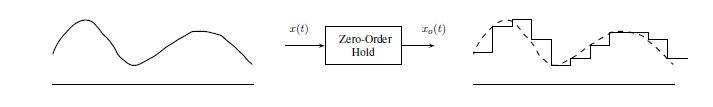
\includegraphics[scale=0.450]{Figures/Sampling/sampling_zoh}
\caption{Sampling using ZOH}
\label{fig:Sampling:sampling_zoh}
\end{figure}

\newpage
\item Implementation:

\begin{itemize}
	\item Let's denote the rectangular pulse we are using by $h(t)$ denoted by:

\begin{equation}
h(t)\, = \, \begin{cases}
1 \quad 0 \, \leq \, t \, \leq \, T_s \\
0 \quad \text{otherwise}
\end{cases}
\end{equation}

\item The $x_{\text{zoh}}$ can be written as:

\begin{equation}
x_{\text{zoh}} \, = \, \displaystyle\sum\limits_{n \, = \, -\infty}^{\infty} x(n) h\left(	t \, - \, n\,T_s \right)
\label{Eq:Sampling:Zoh_eq_1}
\end{equation}

\item Taking advantage from \textcolor{red}{convolution shifting property}: 
Recall that we can obtained a \textcolor{red}{shifted version of a signal} by \textcolor{red}{convolving this signal with a dirac function} so equation (\ref{Eq:Sampling:Zoh_eq_1}) can be further formulated

\begin{equation}
\begin{array}{rcl}
x_{\text{zoh}} \, &=& \, \displaystyle\sum\limits_{n \, = \, -\infty}^{\infty} x(n) \, h\left(	t \, - \, n\,T_s \right) \\ \\		
&=& \, \displaystyle\sum\limits_{n \, = \, -\infty}^{\infty} x(n) \, \times \, \left[ \, \delta \left(	t \, - \, n\,T_s \right) \, * \, h(t) \, \right] \\ 
\end{array}
\label{Eq:Sampling:Zoh_eq_2}
\end{equation}

\item Manipulating the parenthesis of equation (\ref{Eq:Sampling:Zoh_eq_2}):

\begin{equation}
\begin{array}{rcl}
x_{\text{zoh}} \, &=& \, \displaystyle\sum\limits_{n \, = \, -\infty}^{\infty} x(n) \, h\left(	t \, - \, n\,T_s \right) \\ \\		
&=& \, \displaystyle\sum\limits_{n \, = \, -\infty}^{\infty} x(n) \, \times \, \left[ \, \delta \left(	t \, - \, n\,T_s \right) \, * \, h(t) \, \right] \\ \\
&=& \, \displaystyle\sum\limits_{n \, = \, -\infty}^{\infty} \left[\, x(n) \, \times  \, \delta \left(	t \, - \, n\,T_s \right) \, \right] \, * \, h(t)   \\ \\
&=& \,  x_{\delta}(t) \, * h(t)
\end{array}
\label{Eq:Sampling:Zoh_eq_3}
\end{equation}

\begin{figure}[ht]
\centering
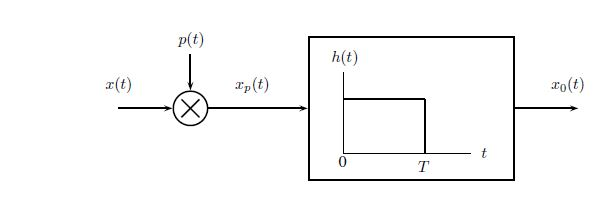
\includegraphics[scale=0.450]{Figures/Sampling/zoh_math}
\caption{Mathematical modeling of the ZOH}
\label{fig:Sampling:zoh_math}
\end{figure}

\item Implication on Spectrum:

\begin{figure}[ht]
\centering
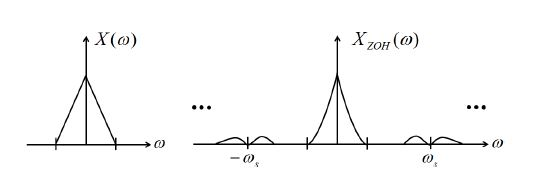
\includegraphics[width = 0.7\textwidth]{Figures/Sampling/zoh_output_spectrum}
\caption{Output of ZOH in the frequency domain}
\label{fig:Sampling:zoh_output_spectrum}
\end{figure}


\begin{itemize}

\item In impulse sampling (see figure \autoref{fig:Sampling:impulse_sampling_spectrum_1}), the spectrum was the same (with the scale factor $\displaystyle\frac{1}{T_s}$), along with the replicate at multiple of $\omega_s$.


\item In ZOH, these \textcolor{red}{replicate are attenuated} due to the low pass nature of the ZOH, which is a good thing since we don't want these images.

\item However, the \textcolor{red}{original spectrum is getting distorted}, and this distortion is controlled by the time sampling we choose to get our values. 

\end{itemize}

\end{itemize}

\item Antimaging-filter: to smooth the effect of the ZOH

\begin{figure}[ht]
\centering
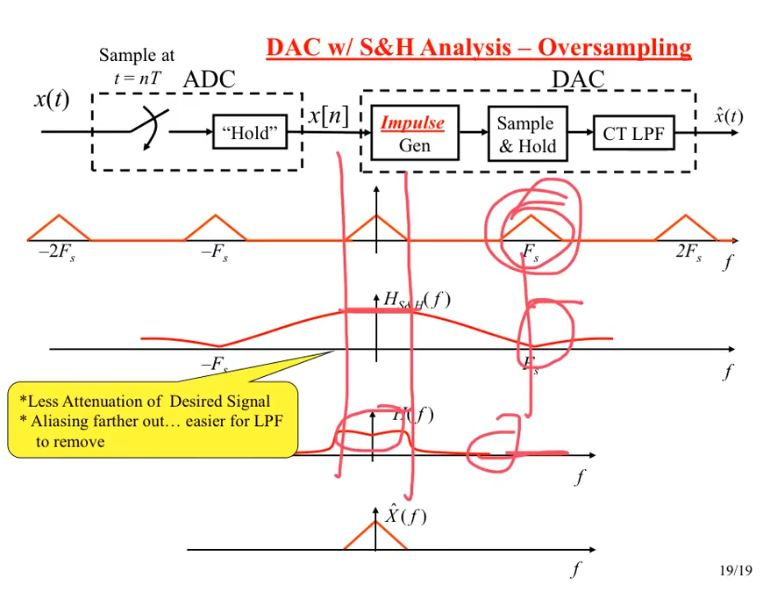
\includegraphics[width = 0.7\textwidth]{Figures/Sampling/oversampling_benefits}
\caption{Over sampling Benefits}
\label{fig:Sampling:oversampling_benefits}
\end{figure}

\begin{itemize}

\item Make the frequency response of the ZOH system more flat in the pass band

\item Easier transition band design for the smoothing filter

\end{itemize}

\item Didn't Grasp yet: people do \textcolor{red} {resampling}(upsampling and Multirate sampling techniques)at $x[n]$ to make the design more easier (didn't do it yet)

\end{itemize}

\end{frame}
